\documentclass[16pt,a4paper]{report}
\usepackage[a4paper, mag=1000, left=2.5cm, right=1cm, top=2cm, bottom=2cm, headsep=0.7cm, footskip=1cm]{geometry}
\usepackage[utf8]{inputenc}
\usepackage[T2A]{fontenc}
\usepackage[english,russian]{babel}
\usepackage{hyperref}
\usepackage{graphicx}
\usepackage{soul}
\usepackage{wrapfig}
\usepackage{float,subcaption}
\graphicspath{ {./} }
%\usepackage{gensymb}

\usepackage{fancyhdr}
\begin{document}
\pagestyle{fancy}
\title{Решение комплексных задач по астрономии}
\author{Головизнин Д.И.}
\fancyhf{}
\fancyhead[R]{Решение комплексных задач по астрономии}
\fancyfoot[L]{\thepage}
\maketitle
\tableofcontents
\newpage
\chapter{Необходимые сведения.}
\section{Градусы, минуты, секунды}
Исторически сложилось, что в окружности содержится 360 градусов. В каждом градусе (${\circ}$) - 60 минут ('), в каждой минуте 60 секунд ("). Соответственно для перевода нужно либо делить на 60, либо умножать на 60. 

\section{Полезные сведения о прямоугольном треугольнике}
Прямоугольный треугольник - достаточно удобная фигура. Ниже перечислена часть тех преимуществ, которые может дать прямоугольный треугольник.
\begin{enumerate}
    \item Легко достраивается до прямоугольника
    \item Формула для нахождения последнего из углов: $90^{\circ} - \alpha = \beta$
    \item Достаточно легко сформулировать трактовки $\sin \textrm{, }\cos\textrm{, } \tan$. Так синус в прямоугольном треугольнике - это отношение противолежащего катета к гипотенузе, косинус - прилежащего к гипотенузе, а тангенс - противолежащего к прилежащему. Выписав любое из отношений и домножив так, чтобы знаменатель и равенство поменялись местами, можно получить формулу для одной из сторон треугольника.
    \item Медиана из прямого угла к гипотенузе - равна половине гипотенузы
\end{enumerate}
\section{Радианная мера угла}
1 радиан - это угол, соответствующий дуге, длина которой равна её радиусу. Считается более естественной (сравнивая с градусами) мерой углов.$$1 \textrm{ Рад} \approx 57,3^{\circ} $$
Чтобы перевести градусы в радианы и обратно, достаточно помнить, что в окружности содержится $2\pi$ радиан и 360 градусов. Поделив одно на другое и умножив на необходимое, получится перевод.

Особенностью является тот факт, что при малых углах, выраженных в радианах, функции $\tan$ и $\sin$ возращают примерно равные самому углу значения.
$$x - \textrm{малый угол в радианной мере;} \sin{x} \approx x \textrm{ и } \tan{x} \approx x$$
\section{Кривые второго порядка}
\subsection{Эллипс}
\begin{figure}[H]
    \centering
    \begin{subfigure}{0.65\textwidth}
        \centering
        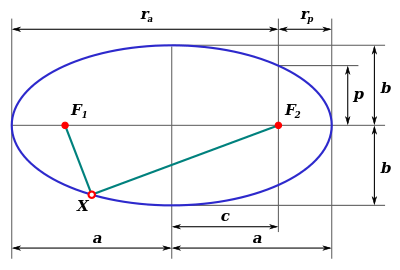
\includegraphics[width=0.65\textwidth]{400px-Ellipse_parameters_3.svg.png}
        \caption{Параметры Эллипса.}
        \label{fig:first}
    \end{subfigure}    
    \qquad
\end{figure}
Это замкнутая геометрическая фигура, обладает эксцентриситетом $e < 1$

Полезные знания и формулы
\begin{enumerate}
    \item Эллипс обладает большой ($a$) и малой полуосью ($b$)
    \item Фокальным расстоянием ($c$) называют полурасстояние между его фокусами
    \item Эксцентриситет считается по формуле $e = \frac{c}{a} = \sqrt{1-\frac{b^2}{a^2}}$
    \item Апоцентр: $a_a = a (1+e)$
    \item Перицентр: $a_p = a (1-e)$
    \item Площадь эллипса: $S = \pi ab = \pi a^2\sqrt{1-e^2}$
\end{enumerate}
\subsection{Окружность}
Окружность - это частный случай эллипса, когда эксцентриситет $e$ = 0
\begin{enumerate}
    \item Формула площади переписывается в $S = \pi r^2$
    \item Длина окружности $L = 2\pi r $
    \item Идея единичной окружности (с $r=1$) удобна и используется в тригонометрии
\end{enumerate}
\subsection{Парабола}
\begin{figure}[H]
    \centering
    \begin{subfigure}{0.5\textwidth}
        \centering
        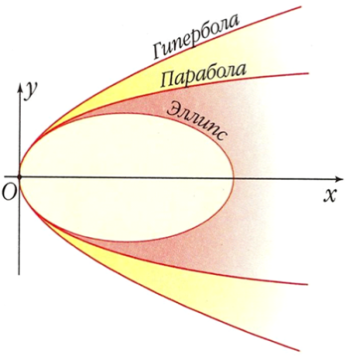
\includegraphics[width=0.5\textwidth]{23250_html_71aca189.png}
        \caption{Парабола.}
        \label{fig:first}
    \end{subfigure}    
    \qquad
\end{figure}
Парабола — геометрическое место точек, равноудалённых от данной прямой
(называемой директрисой параболы) и данной точки (называемой фокусом
параболы). Обладает эксцентричитетом равным 1. При этом не обладает большой и малой полуосью.
Известным примером параболы является квадратичная функция одной переменной.
\subsection{Гипербола}
Гипербола — геометрическое место точек евклидовой плоскости, абсолютное
значение разности расстояний от которых до двух выделенных
называемых фокусами, постоянно и равно удвоенной действительной полуосигиперболы.
Эксцентрисите больше 1, обладает вершинами (ближайшие к друг другу точки). Известный пример - график функции $y = \frac{k}{x}$
\section{Движение по кругу}
$\nu$ - частота оборотов, измеряется в Герц [Гц], $T$ - Период обращения. Частота и период обращения связаны обратной пропорцией $$T = \frac{1}{\nu}$$
$\omega$ - угловая скорость, единица измерения - Радиан
$$\omega = \frac{\Delta \phi}{\Delta t}=2\pi\nu$$
$$U = \omega R$$
\chapter{Размеры и расстояния в астрономии}
\section{Суточный, горизонтальный и годичный параллаксы.}
\subsection{Теория}
%\begin{wrapfigure}{r}{0.25\textwidth} %this figure will be at the right
%    \centering
%    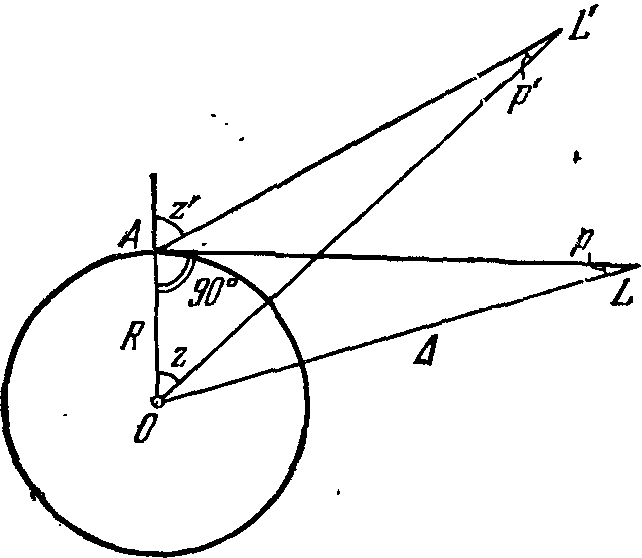
\includegraphics[width=0.25\textwidth]{sutochny_horiz_parallaks.png}
%\end{wrapfigure}

Представим, что у нас есть светило $L'$. Наблюдать за небесными светилами можно с разных мест Земли и для разных мест, и получать разные данные. Поэтому нужно прийти к чему-то единому, а именно направлению из центра Земли к светилу $L'$. Если вторым направлием выступает луч из какой-то точки на Земле к светилу $L'$, то угол между этими двумя направлениями $\angle{AL'O}$ является суточным параллаксом $p'$. 

Теперь представим, что светило $L$ видно из точки $A$ прямо на горизонте. Суточный параллакс $p$ принимает своё максимальное значение и называется горизонтальным параллаксом.
Горизонтальный параллакс удобен для вычисления некоторых расстояний до некоторых объектов Солнечной Системы, так как два направления и базис (радиус Земли) выступают в качестве прямоугольного треугольника. Звёзды будут иметь уже крайне низкие значения.
\begin{figure}[H]
    \centering
    \begin{subfigure}{0.4\textwidth}
        \centering
        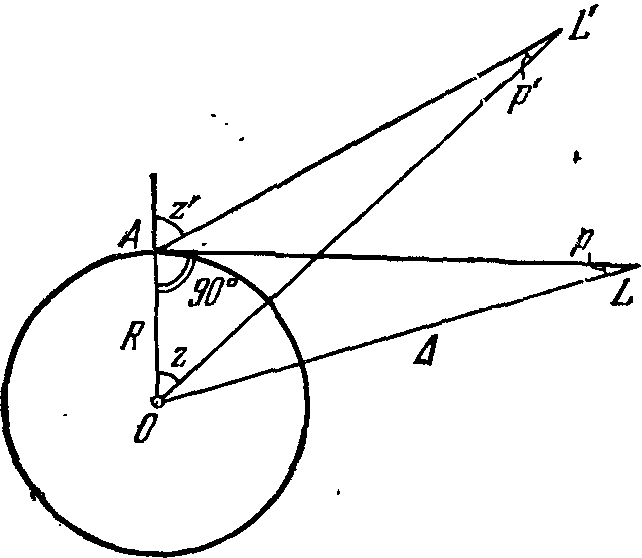
\includegraphics[width=0.5\textwidth]{sutochny_horiz_parallaks.png}
        \caption{Суточный и горизонатльный}
        \label{fig:first}
    \end{subfigure}    
    \qquad
    \begin{subfigure}{0.4\textwidth}
        \centering
        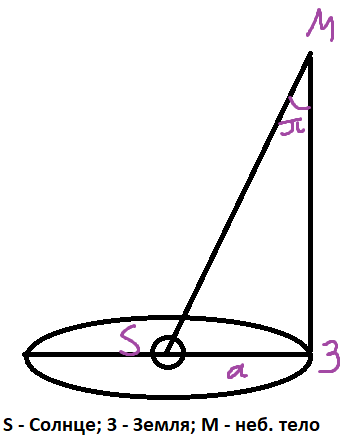
\includegraphics[width=0.3 \textwidth]{godychny_changed_parallaks.png}
        \caption{Годичный}
        \label{fig:second}
    \end{subfigure}    
    \caption{Параллаксы.n}
    \label{fig:enter-label}
\end{figure}




Годичным параллаксом $\pi$ называют угол под которым со звезды был бы виден средний радиус земной орбиты $a$, при условии, что направление на звезду перпендикулярно радиусу $a$.
%Изображение Годичного параллакса 
Годичный параллакс может использоваться для измерения расстояний до звёзд. Также имеет куда более выгодный базис. 

\subsection{Практика}
\begin{enumerate}
    \item [1.1.]Докажите, что Горизонтальный параллакс - максимальный суточный параллакс \emph{(3 балла)}
    \item [1.2.]Вычислите расстояние от Земли до Луны \emph{(1 балл)}
    \item [1.3.] (2.83) Какая звезда и во сколько раз ближе к нам - Денеб ($\alpha$ Лебедя), расстояние до которого 1400 св. лет, или Денебола ($\beta$ Льва), годичный параллакс которой равен 0,090" \emph{(2 балла)}
    \item [1.4.] (2.85 - МОШ-1951) Параллакс Солнца $8,80"$, а параллакс звезды 0,44". Во сколько раз эта звезда дальше от Земли, чем Солнце? Нельзя использовать $a_cp$ \emph{(2 балла)}
\end{enumerate}

\section{Парсек, его связь с астрономической единицей и световым годом.}
\subsection{Теория}
Одной из основных единиц расстояний, в астрономии принят парсек (пк) - расстояние, соответствующее годичному параллаксу в $1"$. Исходя из определения, $$1 \textrm{ пк} = \frac{1 \textrm{ а.е.}}{\tan{1\textrm{''}}} \approx \frac{1}{\frac{1 * \pi}{180^{\circ}}} \approx 206265 \textrm{ а.е.}$$
Если подставить вместо астрономических единиц - световые года, то и ответ будет в световых годах.
$$1 \textrm{ пк} = 206265 \textrm{ а.е.} = 3,26 \textrm{ св.года}$$

Если астрономическая единица используется в пределах Солнечной системы, то парсек и световой год используются до небесных тел за пределами Солнечной системы. В таком случае:
$$\Delta = \frac{1}{\pi} \textrm{пк и } \Delta = \frac{3,26}{\pi}\textrm{ световых лет}  $$
Обратите внимание, что под $\pi$ понимается значение в секундах, но при вычислении числитель и знаменатель должны быть либо в числовых значениях оба, либо в секундах оба
\subsection{Практика}
\begin{enumerate}
    \item [1.5.] (2.80) Расстояние до звезды Бетельгейзе составляет 200 пк. Чему равен её параллакс? \emph{(1 балл)}
    \item [1.6.] (2.79) Чему равно расстояние до звезды в парсеках, если её годичный параллакс равен $0,16"$\emph{(1 балл)}
    \item [1.7.]Выразите расстояние из задачи 2 в километрах и световых годах \emph{(1 балл)}
    \item [1.8.] Ближайшая к Солнцу звезда "Проксима Центавра" имеет годичный параллакс $\pi$ = 0,772". Найдите расстояние от нас до ближайшей звезды, выразите его в парсеках и световых годах. \emph{(1 балл)}
    \item [1.9.] Докажите, что формула $\Delta = \frac{1}{\pi }$ - справедлива для нахождения расстояния в парсеках для небесных тел за пределеами Солнечной системы \emph{(3 балла)}
\end{enumerate}
\section{Угловой размер небесных объектов. Связь линейных и угловых размеров объекта, видимого под малым углом.}
\subsection{Теория}
\begin{wrapfigure}{r}{0.25\textwidth} %this figure will be at the right
    \centering
    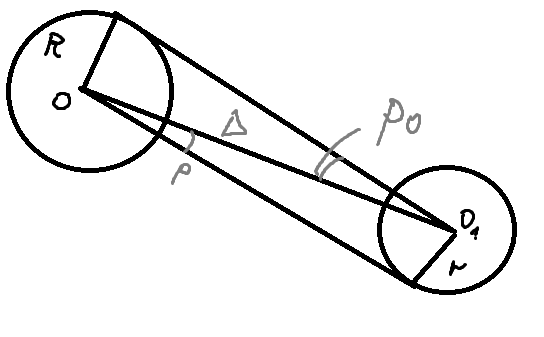
\includegraphics[width=0.25\textwidth]{kismereniu.png}
\end{wrapfigure}
Угловым диаметром является угол, под которым с Земли виден диаметр небесного тела. Если известен угловой диаметр, то можно вычислить его линейный диаметр. Из геометрических соображений ($p_0$ - горизонтальный экваториальный параллакс светила, $p$ - угловой радиус светила) $r = \Delta \sin{p}; R_0 = \Delta \sin{p_0}$. Если выразить $\Delta$ в первой формуле и подставить вместо неё вторую формулу, то мы получим равенство отношений, из которого выразим $$r = \frac{\sin{p}}{\sin{p_0}}R_0$$
Из-за малости углов $p$ и $p_0$, формула сокращается до: $$r = \frac{p}{p_0}R_0$$

Также всё ещё возможно использовать прямоугольный треугольник для вычилений, если известны 2 из 3 параметров. Из-за малых углов синус и тангенвс примерно равны самому углу, что упрощает задачу вычисления.
\subsection{Практика}
\begin{enumerate}
    \item [1.10.] Определите угловой размер Солнца для наблюдателя с Земли. Орбиту Земли считать круговой, а размер Солнца - известным (радиус - 695500 км) \emph{(1 балл)}
    \item [1.11.] Определить линейные размеры Луны, если горизонтальный параллакс равен 57', радиус Земли - 6378 км, а угловой диаметр 31'05'' \emph{(1 балл)}
\end{enumerate}
\chapter{Небесная механика}
\section{Синодический и сидерические периоды}
Промежуток времени для полного оборота вокруг зведы называется Сидерическим периодом обращения ($T$); Промежуток времени между двумя одноимёнными конфигурациями называется Синодическим периодом ($S$)
Для нижней планеты: $$\frac{1}{S} = \frac{1}{T} - \frac{1}{T_{\textrm{з}}}$$
Для верхней планеты: $$\frac{1}{S} = \frac{1}{T_{\textrm{з}}}-\frac{1}{T}$$
Универсальная формула: $$S = \frac{T_{\textrm{з}}T}{|T-T_{\textrm{з}}|}$$
Эти формулы принято называть Уравнениями синодического движения
\section{Закон Всемирного Тяготения}
Каждая частица притягивает каждую другую частицу во Вселенной с силой, прямо пропорциональной произведению их масс и обратно пропорциональной квадрату расстояния между их центрами.
$$\vec{F_t} = G \frac{M*m}{R^2}$$
Из закона Всемирного тяготения выводятся многие полезные формулы, включая формулу Первой Космической скорости.
\section{Законы Кеплера (эмпирические)}
\subsection{Первый закон Кеплера}
Все планеты движутся по эллиптическим орбитам, в одном из фокусов которых находится Солнце.
Как следствие, формулы эллипса - применимы. 
$$e= \frac{c}{a}$$
\subsection{Второй закон Кеплера}
Радиус-вектор планеты за равные промежутки времени заметает равные площади
$$\frac{dS}{dt} = const = \frac{S_ell}{T} = \frac{\pi ab}{T}$$
\subsection{Третий закон Кеплера}
Квадраты периодов обращения планет относятся, как кубы больших полуосей их орбит.
$$\frac{T_1^2}{T_2^2} = \frac{a_1^3}{a_2^3}$$
\subsection{Гомановская траектория}
\begin{wrapfigure}{l}{0.4\textwidth} %this figure will be at the right
    \centering
    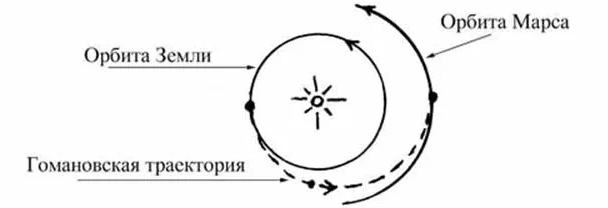
\includegraphics[width=0.4\textwidth]{goman.png}
\end{wrapfigure}
Эклиптическая орбита для перехода между двумя орбитами. Считается энергоэффективной, так как нужны всего два импульса (для входа и схода на траекторию). В простейшем случае она пересекает эти две орбиты в апоцентре и перицентре и является полуэллипсом.

Третий закон Кеплера в данном случае применим, например, при сравнении с Земной орбитой (при этом удобно использовать в качестве $T$ - 1 год, а в качестве $a$ - 1 а.е..
\section{Обобщение законов Кеплера Ньютоном}
В связи с тем, что каждая планета испытывает притяжение других тел - происходят возмущения
\newcounter{foo}
\setcounter{foo}{1} 
\begin{enumerate}
    \item [\Roman{foo} З.К.] - Тело может двигаться по следующим траекториям: эллипс, парабола, гипербола \setcounter{foo}{2}
    \item [\Roman{foo} З.К.] - Без изменений \setcounter{foo}{3}
    \item [\Roman{foo} З.К.] - Добавляет в отношения между телами (планетами) влияние массивного тела (Солнца) $$\frac{T_1^2(M_c + m_1)}{T_2^2(M_c + m_2)}=\frac{a_1^3}{a_2^3}$$
\end{enumerate}
\section{Практика}
Задания:
\begin{enumerate}
    \item [2.1.] Марс в 1,5 раза дальше от Солнца, чем Земля. Какова продолжительность года на Марсе? \emph{(1 балл)}
    \item [2.2.]За 84 года Уран делает один оборот вокруг Солнца. Во сколько раз он дальше от Солнца, чем Земля? \emph{(1 балл)}
    \item [2.3.] Рассчитайте параметры орбиты полёта космического аппарата к Юпитеру (вид траектории, время полёта, угол Земля-Солнце-Юпитер в момент запуска) с точки зрения минимальных энергетических затрат. Орбиты планет считать круговыми. Большая полуось орбиты Юпитера 5,2 а.е., период обращения 11,86 г. \emph{(2 балла)}
    \item [2.4.] (4.61) Синодический период обращения Юпитера при наблюдении с Земли равен 399 сут. Чему равен синодический период обращения Земли при наблюдении с Юпитера? \emph{(2 балла)}
    \item [2.5.] (3.33) Искусственный спутник пролетает на высоте 300км над поверхностью Земли, а потом удаляется от центра нашей планеты на 10000 км. Определите эксцентриситет орбиты спутника.\emph{(2 балла)}
    \item [2.6.] Полет космического аппарата с Земли к некоторой планете по оптимальной траектории занял 6 лет. Что это за планета? \emph{(1 балл)}
    \item [2.7.] (3.41) Маятниковые часы привезли с Земли на Марс. За какое земное время пройдёт 1 час по показаниям этих часов? \emph{(3 балла)}
    \item [2.8.] (3.43) Во сколько раз нужно увеличить скорость движения спутника некоторого центрального тела, чтобы перевести спутник с круговой орбиты на эллиптическую с эксцентриситетом 0,3? Точка изменения скорости должна стать перицентром новой орбиты \emph{(3 балла)}
    \item [2.9.] (4.75) Сколько времени проходит от наибольшой западной элонгации Венеры до её верхнего соединения? \emph{(3 балла)}
    \item[2.10.] (МОШ-2003, 4.72) Пусть внутренняя планета А и внешняя планета Б при наблюдении с Земли имеют одинаковый синодический периож. Чему равен синодический период планеты А при наблюдении с планеты Б? \emph{(3 балла)}
\end{enumerate}
\newpage
\chapter{Движение по орбите}
\section{Теория}
\subsection{Первая космическая скорость и её вывод}
Первая космическая скорость - это минимальная (для заданной высоты над центральным телом) горизонтальная скорость, которую необходимо придать объекту, чтобы он совершал движение по круговой орбите вокруг центрального тела.
$$F = ma$$
$$\frac{mU^2}{R}=\frac{GmM}{R^2} => \frac{\textrm{\st{m}}U^2}{\textrm{\st{R}}}=\frac{G\textrm{\st{m}}M}{R^{\textrm{\st{2}}}} = > U = \sqrt{\frac{GM}{R}}$$
Так как $g = \frac{GM}{R^2}$, то $$U = \sqrt{gR}$$, таким образом посчитать Первую Космическую Скорость у поверхности Земли будет легче и она примерно равна 7900 м/с.
\subsection{Следствия из закона сохранения импульса}
Закон сохранения момента импульса справедлив как для движения по эллипсу, так и по гиперболе и параболе. Следствием этого закона и закона сохранения энергии является интеграл энергии — формула для скорости тела в точке орбиты, удалённой на расстояниецентрального тела с массой M :
$$U = \sqrt{GM(\frac{2}{r}-\frac{1}{a})}$$
Следствием этой формулы являются случаи в апоцентре и перицентре:
$$U_a =\sqrt{\frac{GM(1-e)}{a(1+e)}}$$
$$U_p =\sqrt{\frac{GM(1+e)}{a(1-e)}}$$
\subsection{Альтернативная форма 3-го Закона Кеплера}
Вы уже знаете о $$\frac{T^2}{a^3}=const$$, но есть и альтернативная формула, позволяющая находить массу, радиус планеты или сидерический период, имея хотя бы 2 значения.
$$\frac{GMT^2}{4\pi^2}=R^3$$
\newpage
\section{Практика}
\begin{enumerate}
    \item [3.1] Докажите формулу из 4.1.2. для равномерного движения тела по окружности \emph{(3 балла)}
    \item [3.2.] (3.22) Какую скорость (в км/с) должно иметь космическое тело, чтобы облететь Солнце у самой поверхности? \emph{(1 балл)}
    \item [3.3.] (3.25) Вычислите первую космическую скорость для Марса (масса Марса составляет 0,11 массы Земли, радиус меньше земного примерно в 1,9 раза, а первая космическая скорость для Земли равна 7,9 км/с). Запрещено пользоваться справочными материалами для решения этой задачи.\emph{(1 балл)}
    \item [3.4.] (3.38) Чему равна большая полуось геостационарного спутника и скорость, с которой он движется по орбите?\emph{(2 балла)}
    \item [3.5] (3.50) Предположим, что масса Солнца внезапно увеличилась вдвое. Какой эксцентриситет и период обращения будет у Земли? \emph{(3 балла)}
    \item [3.6] (3.51) Предположим, Солнце стало терять массу со скоростью 1 млрд т в секунду. На какое расстояние удалится от него Земля за 1 год? Изначально орбиту Земли считайте круговой. \emph{(3 балла)}
    
\end{enumerate}
\newpage
\chapter{Приложение}
\section{Константы}
\begin{enumerate}
    \item $R_0$ = 6378 км (Экваториальный радиус Земли)
    \item $p_l$ = $57'$ (Средний горизонтальный параллакс Луны)
    \item $a_cp$ = 1 а.е. = $1,496 * 10^{11}$ м (Средний радиус орбиты Земли)
    \item $c$ = $2.998 * 10^8$ м/с (Скорость света в вакууме)
    \item Пк = 206265 a.e. (Парсек в световых годах)
    \item $G = 6.674 * 10^{-11} \textrm{м}^3*\textrm{кг}^{-1}*c^{-2}$ (Гравитационная Постоянная)
\end{enumerate}
Ссылка на константы Регионального Этапа (пожалуйста, не используйте, если задача предполагает решение без данных констант)
\href{https://всош.цпм.рф/upload/files/Arhive_tasks/2022-23/reg/astr/spdata-astr-9-11-reg-22-23.pdf}{Ссылка}
\section{Практика всего занятия}
\begin{enumerate}
    \item [1.1.] Докажите, что Горизонтальный параллакс - максимальный суточный параллакс \emph{(3 балла)}
    \item [1.2.] Вычислите расстояние от Земли до Луны \emph{(1 балл)}
    \item [1.3.] (2.83) Какая звезда и во сколько раз ближе к нам - Денеб ($\alpha$ Лебедя), расстояние до которого 1400 св. лет, или Денебола ($\beta$ Льва), годичный параллакс которой равен 0,090" \emph{(2 балла)}
    \item [1.4.] (2.85 - МОШ-1951) Параллакс Солнца $8,80"$, а параллакс звезды 0,44". Во сколько раз эта звезда дальше от Земли, чем Солнце? Нельзя использовать $a_{cp}$ \emph{(2 балла)}
    \item [1.5.] (2.80) Расстояние до звезды Бетельгейзе составляет 200 пк. Чему равен её параллакс? \emph{(1 балл)}
    \item [1.6.] (2.79) Чему равно расстояние до звезды в парсеках, если её годичный параллакс равен $0,16"$\emph{(1 балл)}
    \item [1.7.] Выразите расстояние из задачи 2 в километрах и световых годах \emph{(1 балл)}
    \item [1.8.] Ближайшая к Солнцу звезда "Проксима Центавра" имеет годичный параллакс $\pi$ = 0,772". Найдите расстояние от нас до ближайшей звезды, выразите его в парсеках и световых годах. \emph{(1 балл)}
    \item [1.9.] Докажите, что формула $\Delta = \frac{1}{\pi }$ - справедлива для нахождения расстояния в парсеках для небесных тел за пределеами Солнечной системы \emph{(3 балла)}
    \item [1.10.] Определите угловой размер Солнца для наблюдателя с Земли. Орбиту Земли считать круговой, а размер Солнца - известным (радиус - 695500 км) \emph{(1 балл)}
    \item [1.11.] Определить линейные размеры Луны, если горизонтальный параллакс равен 57', а угловой диаметр 31'05'' \emph{(1 балл)}
    \item [2.1.] Марс в 1,5 раза дальше от Солнца, чем Земля. Какова продолжительность года на Марсе? \emph{(1 балл)}
    \item [2.2.]За 84 года Уран делает один оборот вокруг Солнца. Во сколько раз он дальше от Солнца, чем Земля? \emph{(1 балл)}
    \item [2.3.] Рассчитайте параметры орбиты полёта космического аппарата к Юпитеру (вид траектории, время полёта, угол Земля-Солнце-Юпитер в момент запуска) с точки зрения минимальных энергетических затрат. Орбиты планет считать круговыми. Большая полуось орбиты Юпитера 5,2 а.е., период обращения 11,86 г. \emph{(2 балла)}
    \item [2.4.] (4.61) Синодический период обращения Юпитера при наблюдении с Земли равен 399 сут. Чему равен синодический период обращения Земли при наблюдении с Юпитера? \emph{(2 балла)}
    \item [2.5.] (3.33) Искусственный спутник пролетает на высоте 300км над поверхностью Земли, а потом удаляется от центра нашей планеты на 10000 км. Определите эксцентриситет орбиты спутника.\emph{(2 балла)}
    \item [2.6.] Полет космического аппарата с Земли к некоторой планете по оптимальной траектории занял 6 лет. Что это за планета? \emph{(1 балл)}
    \item [2.7.] (3.41) Маятниковые часы привезли с Земли на Марс. За какое земное время пройдёт 1 час по показаниям этих часов? \emph{(3 балла)}
    \item [2.8.] (3.43) Во сколько раз нужно увеличить скорость движения спутника некоторого центрального тела, чтобы перевести спутник с круговой орбиты на эллиптическую с эксцентриситетом 0,3? Точка изменения скорости должна стать перицентром новой орбиты \emph{(3 балла)}
    \item [2.9.] (4.75) Сколько времени проходит от наибольшой западной элонгации Венеры до её верхнего соединения? \emph{(3 балла)}
    \item[2.10.] (МОШ-2003, 4.72) Пусть внутренняя планета А и внешняя планета Б при наблюдении с Земли имеют одинаковый синодический периож. Чему равен синодический период планеты А при наблюдении с планеты Б? \emph{(3 балла)}
    \item [3.1] Докажите формулу из 4.1.2. для равномерного движения тела по окружности \emph{(3 балла)}
    \item [3.2.] (3.22) Какую скорость (в км/с) должно иметь космическое тело, чтобы облететь Солнце у самой поверхности? \emph{(1 балл)}
    \item [3.3.] (3.25) Вычислите первую космическую скорость для Марса (масса Марса составляет 0,11 массы Земли, радиус меньше земного примерно в 1,9 раза, а первая космическая скорость для Земли равна 7,9 км/с). Запрещено пользоваться справочными материалами для решения этой задачи.\emph{(1 балл)}
    \item [3.4.] (3.38) Чему равна большая полуось геостационарного спутника и скорость, с которой он движется по орбите?\emph{(2 балла)}
    \item [3.5] (3.50) Предположим, что масса Солнца внезапно увеличилась вдвое. Какой эксцентриситет и период обращения будет у Земли? \emph{(3 балла)}
    \item [3.6] (3.51) Предположим, Солнце стало терять массу со скоростью 1 млрд т в секунду. На какое расстояние удалится от него Земля за 1 год? Изначально орбиту Земли считайте круговой. \emph{(3 балла)}
\end{enumerate}
\begin{flushright}
\emph{51 балл}
\end{flushright}
\newpage
\section{Указания к решению заданий практики}
Всегда помните, что указания к решению не являются полноценными решениями.


\begin{enumerate}
    \item [1.1.] Возможный вариант подхода к решению: Выбрать произвольную точку $T$ (Наблюдатель) на поверхности Земли. Представить Землю как круг с центром $O$ и точкой $T$ на окружности, выбрать произвольно точку $B$ (небесное тело) в пределах поля зрения Наблюдателя. Провести 2 касательные из $B$ к окружности с точками $A$ и $A'$ (пояснить, что это горизонт и он существует в любой ситуации), заметить осевую симметрию по $BO$. А также заметить, что наблюдатель $T$ окажется внутри угла $\angle{ABA'}$ (требуется объяснение). Довести решение задачи можно через прямоугольные треугольники $ABO$ и $ABC'$ , где отрезок $BC'$ лежит на луче $BT$.
    
    
     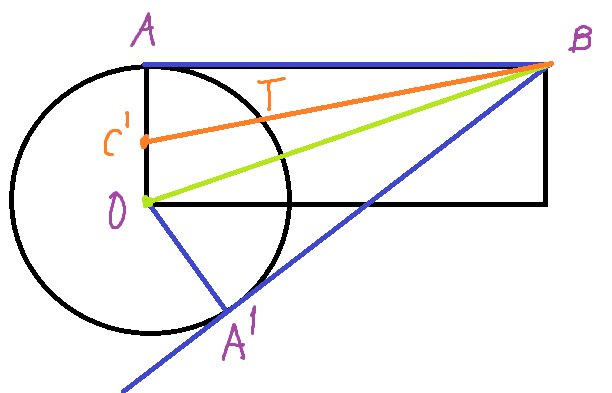
\includegraphics[scale=0.25]{task1.png}
    \item [1.2.]Чистый прямоугольный треугольник. $$ L = \frac{R_0}{\sin{p_l}} = 384683,396 \textrm{ км}$$
    \item [1.3.] Задача состоит из правильного перевода световых лет в СИ (или СИ в световые годы). Также стоит досматривать за правильным вводом секунд в калькулятор (если используется). $$\frac{R_{deneb}}{R_{denebola}} = \frac{1400*(c*T_{tp}*86400)}{\frac{a}{\sin{\pi}}} \approx 39 \textrm{ раз}$$
    \item [1.4.] Важно понимать о каком параллаксе идёт речь в кажом из случаев. Горизонтальный для Солнца, годичный для звезды. $$l_{s} = \frac{R_0}{\sin{p}}; L = \frac{l_{s}}{\sin{\pi}}; \frac{L}{l_{s}} = \frac{1}{\sin{\pi}} = 468783,6506 \approx 469000 \textrm{ раз}$$
    \item [1.5.] Используем обратную формулу $\pi  = \frac{1}{\Delta} = 5*10^{-3}"$
    \item [1.6.] Используем прямую формулу $$\Delta = \frac{1}{\pi } = 6,25 $$
    \item [1.7.] Для киллометров просто умножить $6,25 * 206265 * 1,496*10^8 \approx 1,93 * 10^{14}$ км, для световых лет достаточно заменить 1 в числителе на 3,26 = 20,375 св. лет
    \item [1.8.] 1,3 пк и 4,2 световых года. Подстановка в формулы.
    \item [1.9.] Представим 2 годичных параллакса с $1"$ ($p$) и $p'$. Тогда отношение расстояний $$\frac{r}{r'} = \frac{\frac{a}{\tan{p}}}{\frac{a}{\tan{p'}}} = \frac{\tan{p'}}{\tan{p}}$$ Далее идёт поправка на то, что $p$ и $p'$ - малые, тогда формула становится отношением углов в радианной мере и перевод в радианы - сокращаются. Вместо $r$ подставляется 1 пк, а вместо $p$ - $1"$. Тогда $$r' = \frac{1\textrm{''} * 1 \textrm{ пк}}{p \textrm{''}}$$
    \item [1.10.] Прямоугольный треугольник: $\alpha = \arctan{\frac{D}{a}}; 2\alpha = p \approx 0.53^{\circ}$
    \item [1.11.] $$\frac{\sin{(31'05'' / 2)}}{\sin{57'}}*R_0 = 1746 \textrm{ км}$$
    \newpage
    \item [2.1.] $$T=T_{\textrm{e}}\frac{a_m}{a_e}\sqrt{\frac{a_m}{a_e}} \approx 1.84 \textrm{г}$$
    \item [2.2.] $$a_u = a_e \sqrt[3]{\frac{T_u^2}{T_e^2}} \approx 19,2 \textrm{а.е.}$$
    \item [2.3.] $\approx 97^{\circ}$ \begin{figure}[H]
    \centering
    \begin{subfigure}{0.8\textwidth}
        \centering
        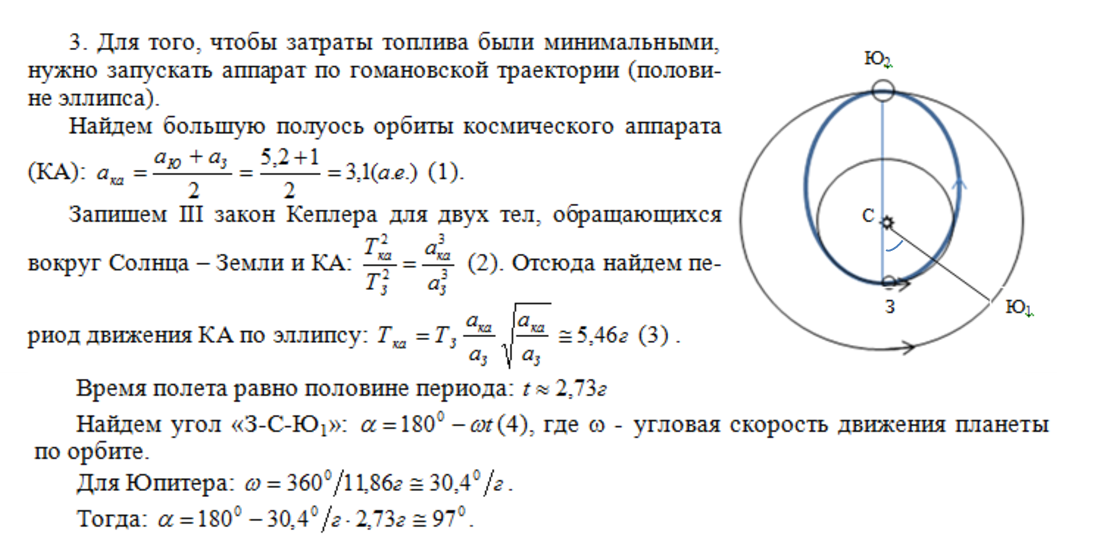
\includegraphics[width=0.9\textwidth]{2.3.PNG}
        \caption{2.3.}
        \label{fig:first}
    \end{subfigure}    
    \qquad
\end{figure}
    \item [2.4.] 399 суток
    \item [2.5.] $\approx 0.2$
    \item [2.6.] Сатурн
    \item [2.7.] За 1.6 часа
    \item [2.8.] В $\sqrt{1,3} \approx 1,14 \textrm{раза}$
    \item [2.9.] 225 земные сутки
    \item [2.10] $0,5S$ 
    \item [3.1.] Из Закона Всемирного тяготения и движения по кругу
    \item [3.2.] $\approx 437 \textrm{км/с}$ 
    \item [3.3.] $\approx 3,6 \textrm{км/с}$
    \item [3.4.] $\approx 3 \textrm{км/с}$ и $\approx 42300 \textrm{км}$
    \item [3.5.] 0,5 и $\approx 141 \textrm{суток}$
    \item [3.6.] $\approx 2,4 \textrm{м}$
\end{enumerate}
\end{document}